\ifdefined \wholebook \else\documentclass[oneside]{book}\usepackage{EdlBook}\graphicspath{{figures/}}
\addto\captionsicelandic{\renewcommand{\chaptername}{Kafli}}
%\setsecnumdepth{chapter}
\begin{document}
%%%
%
\setcounter{chapter}{0} % one less than this chapter
%
%%%
\fi
%%%%%%%%%%%%%%%%%%%%%%%%%%%%%%%%
%      CHAPTER TEXT GOES BELOW
%%%%%%%%%%%%%%%%%%%%%%%%%%%%%%%%

\renewcommand{\thefigure}{\arabic{figure}}
\counterwithout{equation}{chapter}


\chapter{Einingar}

\section{Alþjóðlega einingakerfið}

Alþjóðlega einingakerfið eða SI-kerfið hefur sjö grunneiningar sem sjá má í töflu (\ref{tafla:einingakerfi}). Við ritum oft forskeyti fyrir framan stærðir SI-kerfisins til að lýsa betur stærðargráðu hlutarins sem um ræðir. Forskeytin má sjá í töflu (\ref{tafla:forskeyti}).


\begin{table}[H]
\centering
\begin{minipage}[t]{0.5\linewidth}
\centering

\begin{tabular}{|c|c|c|}
\hline
\textbf{Mælistærð} & \textbf{Skammstöfun} & \textbf{Eining} \\
\hline
Lengd & m & Metri \\
Tími & s & Sekúnda \\
Massi & kg & Kílógramm  \\
Hiti & K  & Kelvin \\
Efnismagn & mol & Mól \\
Rafstraumur  & A    & Amper  \\
Ljósstyrkur  & cd & Kandela \\
\hline
\end{tabular}
\caption{Grunneiningar alþjóðlega einingakerfisins.}
\label{tafla:einingakerfi}
\end{minipage}\hfill
\begin{minipage}[t]{0.5\linewidth}
\centering
\begin{tabular}{|c|c|c|}
\hline
\textbf{Forskeyti} & \textbf{Skammstöfun} & \textbf{Gildi} \\
\hline
tera & T & $10^{12}$ \\
giga & G & $10^9$ \\
mega & M & $10^6$  \\
kilo & k  & $10^3$ \\
hecto & h & $10^2$ \\
deka  & da    & $10$  \\
deci  & d & $10^{-1}$ \\
centi  & c & $10^{-2}$ \\
milli  & m & $10^{-3}$ \\
micro  & $\mu$ & $10^{-6}$ \\
nano  & n & $10^{-9}$ \\
pico  & p & $10^{-12}$ \\
femto  & f & $10^{-15}$ \\
\hline
\end{tabular}
\caption{Helstu forskeyti alþjóðlega einingakerfisins.}
\label{tafla:forskeyti}
\end{minipage}
\end{table}


Til dæmis tölum við um millimetra (mm), kílógrömm (kg) og nanósekúndur (ns). Við bætum þessum forskeytum líka fyrir framan mælistærðir sem ekki eru grunneiningar SI-kerfisins. Til dæmis tölum við um terabæti (TB), desilítra (dL) og megaviku (MV). Takið eftir því að grunneiningin fyrir massa, kílógramm, er skilgreind með forskeyti ólíkt hinum grunneiningum SI-kerfisins. Út frá þessum einingum getum við skilgreint allar afleiddar stærðir SI einingakerfisins, t.d.~getum við skilgreint lítrann þannig að $\SI{1000}{L}$ jafngildi $\SI{1}{m^3}$.

\section{Staðalform og markverðir stafir}

Allar mælingar í eðlisfræði fela í sér einhverja óvissu. Við getum til dæmis verið með óvissu vegna þess að mælitækin okkar eru ekki nógu góð, t.d.~er mesta nákvæmni sem venjuleg reglustika getur sýnt upp á $\SI{1}{mm}$.
Það þýðir að ef við mælum stærð með reglustiku sem $\SI{12.3}{cm}$ þá erum við í rauninni að fullyrða að raunveruleg lengd reglustikunnar sé því næst að vera $\SI{12,3}{cm}$ miðað við mælikvarða reglustikunar.
Ef við hefðum notað nákvæmara mælitæki, eins og t.d. millimetramæli sem hefur mælióvissu upp á $\SI{0.1}{mm}$ þá hefðum við kannski sagt að lengd reglustikunnar væri $\SI{12,34}{cm}$ (og þá hefðum við verið að námunda niður miðað við mælingu með reglustikunni). Þannig þegar við segjum að reglustikan hafi lengdina $\SI{12,3}{cm}$ þá erum við í rauninni að fullyrða að hún hafi lengd sem er einhverstaðar inni 
á bilinu frá $\SI{12.25}{cm}$ upp í $\SI{12.35}{cm}$. Svo við erum í rauninni að fullyrða að raunveruleg lengd reglustikunnar sé $\SI{12,30(5)}{cm}$. En þar sem að við hefðum getað farið línuvilt á reglustikunni þegar við framkvæmdum mælinguna þá er öruggara og fallegra að stækka matið okkar á óvissunni og við segjum þess vegna iðulega að lengdin sé gefin með $\SI{12.3(1)}{cm}$ , þ.e.~við tvöföldum oftast mælióvissuna til öryggis. \\

Það tíðkast í raunvísindum að setja fram mælingar á staðalformi. Segjum að við höfum einhverja tölu $a$ sem hefur $n$ marktæka stafi. Þegar við setjum töluna $a$ fram á staðalformi þá skrifum við hana þannig að:
\begin{align*}
    a = b_1, b_2 \cdots b_n \cdot 10^{c} \, \, [k]
\end{align*}
þar sem $[k]$ táknar samsetningu af grunneiningum SI-kerfisins. Sem dæmi þá myndu $\SI{12,3}{cm} = \SI{0,123}{m}$ á staðalformi. Ástæðan er sú að staðalformið hefur ýmsa kosti. Fyrst ber að nefna að það gefur okkur hugmynd um óvissuna í mælingunni. Annar kostur er sá að það verður miklu auðveldara að vinna með tugveldin, þannig sparar maður sér oft mikla inslætti í reiknivélar.

\section{Fermi vandamál}

Ítalski eðlisfræðingurinn og nóbelsverðlaunahafinn Enrico Fermi var þekktur fyrir að geta gefið ótrúlegustu nálganir á flóknum dæmum út frá nánast engum upplýsingum. Sagan segir að þegar fyrsta kjarnorkusprengjan, Trinity, var sprengd, 16. júlí árið 1945 í Los Alamos, Nýju Mexikó, þá hafi Fermi verið búinn að rífa niður blað sem hann sleppti síðan þegar höggbylgjan barst frá sprengjunni. Út frá því hversu langt blaðsnifsin bárust mat hann sem svo að stærð sprengjunnar væri af stærðargráðunni 10 kílótonn af TNT, sem er ekki í fjærri lagi frá viðteknu gildi, 22 kílótonn. Það getur verið mikilvægur eiginleiki að læra slumpreikninga Fermis. Þá brjótum við niður dæmið í mörg minni skref og leysum hvert skref með ágiskun. Útkomman verður síðan merkilega nákvæm. 
Frægt Fermi vandamál (sem hefur t.d.~birst í atvinnuviðtölum hjá Google) er eftirfarandi spurning:

\begin{itemize}
    \item \textit{Hvað eru margir píanóstillarar í Chicago borg?}
\end{itemize}

Nú þurfum við að brjóta niður vandamálið. Í einhverjum skilningi er hægt að segja að því meira sem við brjótum verkefnið niður því nákvæmari veðrur niðurstaðan okkar. Til dæmis gætum við byrjað á því að giska á hversu margir búa yfir höfuð í Chicago. Við gætum giskað á að þar búi um 5 milljón manns (nákvæma talan er samt \SI{2.7}{} milljónir). Við gætum síðan reynt að meta fjölda þeirra sem eiga píanó 
í Chicago borg. Það eru frekar fjölskyldur heldur en einstaklingar sem eiga píanó og það er eflaust svona fimmta hver fjölskylda sem á píanó. Ef hver fjölskylda hefur fjóra einstaklinga þá höfum við að heildarfjöldi píanóa í Chicago borg er:
\begin{align*}
    \explain{5.000.000}{\text{Chicagobúar}} \hspace{0.35cm} \cdot \explain{\frac{1}{4} \cdot \frac{1}{5}}{\text{píanófjölskyldur}} = 250.000.
\end{align*}
Svo í heildina eru 250.000 píanó í Chicago borg. Það þarf síðan að stilla píanó á 5 ára fresti svo það þarf að stilla 50.000 píanó á ári. Ef það tekur 4 tíma að stilla píanó þá nær reyndur píanóstillir að stilla 2 píanó á einum degi miðað við 8 tíma vinnuviku. Hann vinnur síðan í 300 daga á ári með fríum svo einn píanóstillir nær að stilla 600 píanó á ári. En þá eru 50.000/600 = 83 píanóstillarar í Chicago borg. Þetta passar líka ágætlega við það að á Íslandi eru 6 píanóstillarar en $83 \cdot 300.000/5.000.000 \approx 5$.

\section{Víddargreining}


\begin{minipage}{\linewidth}
    

\begin{wrapfigure}{r}{3.5cm}
\vspace{-1cm}
\centering
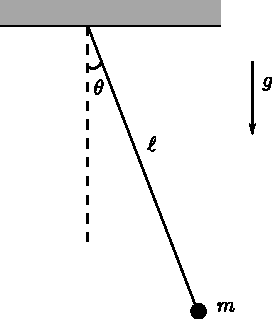
\includegraphics{kaflar/kafli01/figures/pendull.pdf}
\caption{Pendúll, þ.e.a.s.~massi, $m$, sem hangir í bandi af lengd $\ell$ í þyngdarsviði með þyngdarhröðun $g$.}
\label{fig:pendull}
\end{wrapfigure}

Víddargreining er afar öflugt tól sem við munum beita mikið síðar. Það er bæði notað til þess að giska á ný lögmál og til þess að staðfesta að þau lögmál sem við höfum séu samkvæm sjálfum sér. Sem stendur þá þekkið þið ekki nógu mikið af afleiddum einingum (eins og t.d.~eininguna fyrir kraft, Newton, eða eininguna fyrir orku, Joule) og því verður fyrsta umfjöllunin okkar heldur lausleg - í rauninni ætlum við bara að taka eitt dæmi.

\vspace{0.2cm}

Hugsum okkur að við viljum meta sveiflutíma pendúls, $T$. Fyrir þau ykkar sem langar til að spurja: ,,Hvað er pendúll?'' þá mæli ég með að skoða mynd \ref{fig:pendull} hér til hægri. Pendúll er semsagt massi, $m$, sem hangir úr bandi af lengd $\ell$ og sveiflast fram og til baka í þyngdarsviði með þyngdarhröðun $g$. Víddargreining gæti alveg eins heitið einingargreining því það er í rauninni það sem við erum að gera. Við erum að 
pússla saman einingunum á stærðunum þannig að þær passi saman. Það bara vill þannig til að víddargreining hljómar eins og að það sé merkilegra heldur en einingargreining svo við veljum það nafn frekar.
Við ætlum semsagt að skoða víddirnar á eftirfarandi stærðum í þessu dæmi: Massinn $m$, Sveiflutíminn, $T$, lengdin $\ell$ og þyngdarhröðunin $g$. Þegar við viljum taka fram víddirnar þ.e.a.s.~einingarnar á einhverri stærð þá gerum við það með hornklofum, eins og t.d.~í þessu tilviki þá höfum við:
\begin{align*}
    \left[ T \right] = \si{s}, \hspace{1cm} \left[ m \right] = \si{kg}, \hspace{1cm} \left[ \ell \right] = \si{m}, \hspace{1cm} \left[ g \right] = \si[per-mode=fraction]{\metre\per\second\squared}.
\end{align*}
\end{minipage}

Þar sem að einu stærðirnar sem koma fyrir í þessu dæmi eru þessar fjórar þá getum við fullyrt að til séu fastar $\alpha, \beta$ og $\gamma$ þannig að:
\begin{align*}
    T = m^\alpha \ell^\beta g^\gamma
\end{align*}
Reyndar, er þetta tæknilega séð ekki alveg rétt, því það er líka eitthvað hæði á einingarlausa horninu $\theta$ svo tæknilega séð ættum við að segja að til sé fall $f(\theta)$ þannig að:
\begin{align*}
    T = f(\theta) \, m^\alpha \ell^\beta g^\gamma
\end{align*}
Við skulum hunsa fallið $f(\theta)$ í bili og einbeita okkur að því að ákvarða fastana $\alpha, \beta$ og $\gamma$ út frá einingunum. Við tökum núna hornklofa báðum megin (þ.e.a.s~einingar/víddir) og höfum að:
\begin{align*}
    \left[ T \right] = \left[ m \right]^\alpha \left[ \ell \right]^\beta \left[ g \right]^\gamma \iff \si{s} = \si{kg}^\alpha \si{m}^\beta \left(\si[per-mode=fraction]{\metre\per\second\squared}\right)^\gamma
\end{align*}
Ef við tökum núna saman veldin hægra megin og vinstra megin þá sjáum við að:
\begin{align*}
    \si{s}^1 \si{kg}^0 \si{m}^0 = \si{s}^{-2\gamma} \si{kg}^\alpha \si{m}^{\beta + \gamma}
\end{align*}
Með því að bera saman stig og stuðla þá sjáum við að við höfum fengið eftirfarandi jöfnuhneppi:
\begin{align*}
    \begin{cases} -2\gamma = 1 \\
    \alpha = 0 \\
    \beta + \gamma = 0\end{cases} 
\end{align*}
En út frá því ályktum við að lausnin sé $(\alpha, \beta, \gamma) = (0, \frac{1}{2},-\frac{1}{2})$ og því höfum við sýnt að sveiflutíminn hlítur að vera gefinn með:
\begin{align*}
    T = f(\theta) \, \sqrt{\frac{\ell}{g}}.
\end{align*}
Fallið $f(\theta)$ reynist síðan (hefði kannski verið hægt að giska á það?) vera $f(\theta) = 2\pi$ fyrir einfaldan pendúl, en þá er sveiflutíminn gefinn með:
\begin{align*}
    T = 2\pi \sqrt{\frac{\ell}{g}}.
\end{align*}

\newpage

\section{Dæmi}


\subsection*{Einingar, markverðir stafir og staðalform}

\begin{enumerate}[label = \textbf{Dæmi \thechapter.\arabic*.}]

\item Við Evrópubúarnir búum svo vel að hafa alist upp með SI-einingakerfið og notum því metra í daglegu tali. En víðsvegar um heiminn notar fólk aðrar (óheppilegar) lengdareiningar enn þann dag í dag. Við skulum skoða nokkrar þeirra hér í töflu \ref{tafla:einingakerfi2} hér fyrir neðan:

\begin{table}[H]
    \centering
\begin{tabular}{|c|c|c|c|}
\hline

\textbf{Stærð} & \textbf{Enska} &  \textbf{Skammstöfun} & \textbf{Jafngildir} \\
\hline
Þumlungar & Inch & in & \SI{2.54}{cm} \\
Fet & Feet & ft & \SI{30.5}{cm} \\
Álnir & Ell  & el & \SI{49.1}{cm} \\
Yardar & Yard  & yd & \SI{91.44}{cm} \\
Mílur & Mile & mi & \SI{1.609}{km}  \\
\hline
\end{tabular}
\caption{Aðrar einingar sem notaðar eru víðsvegar í heiminum.}
\label{tafla:einingakerfi2}
\end{table}
\vspace{-0.4cm}
Breytið eftirfarandi stærðum yfir á staðalform:

    \begin{tasks}[label = {(\alph*)}, label-format={\bfseries}, label-offset = {0.4cm}](4)
          \task \SI{6}{ft} \SI{6}{in}
          \task \SI{410}{mi}
          \task $120$ álnir vaðmáls
          \task $100$ yards
    \end{tasks}
    
\item Breytið eftirfarandi stærðum yfir á staðalform:

    \begin{tasks}[label = {(\alph*)}, label-format={\bfseries}, label-offset = {0.4cm}](4)
          \task \SI{286.6}{mm}
          \task \SI{760}{mg}
          \task \SI{22.5}{nm}
          \task \SI{62.1}{ps}
    \end{tasks}

\item Þorgeir er mikill hlaupagarpur. Hann lætur alltaf iPodinn sinn mæla vegalengdirnar sem hann hleypur. Því miður kann hann ekki að breyta stillingunum í honum svo iPodinn er alltaf stilltur á mílur. Ef hann ætlar að hlaupa $\SI{16.0}{km}$ hversu margar mílur á hann þá að hlaupa?

\item Hversu margar sekúndur eru í einu ári?

\item Meðalfjarlægðin milli jarðarinnar og sólarinnar kallast stjarnfræðieining og er táknuð með $\SI{1}{AU}$ sem jafngildir $\SI{149.6}{}$ milljón kílómetrum. Setjið fram stjarnfræðieininguna á staðalformi.

\item Ljósár, er þrátt fyrir nafnið, lengdarmælieining og jafngildir vegalengdinni sem ljósið ferðast á einu ári. Ef hraði ljósins er $c = \SI{3.00e8}{m/s}$, hver er þá lengd eins ljósárs, $\SI{1}{ly}$, á staðalformi?

\item Hversu margar stjarnfræðieiningar eru í einu ljósári?

\subsection*{Fermi vandamál}

\item Hversu margir tennisboltar kæmust fyrir inni í flugvél?

\item Hversu margar hárgreiðslur eru útfærðar á hverju ári í Bandaríkjunum?

\item Hversu margir lítrar af vatni eru í Atlantshafinu?

\item Hverjar eru árstekjur Dominos á Íslandi?

\item Hvað eru margir lítrar af vatni í Tjörinni í Reykjavík?

\begin{comment}
\subsection*{Víddargreining}

\item Hæð bolta, $h$, sem fall af tíma, $t$, er gefinn með $h = A + Bt + Ct^2$. Ákvarðið einingar fastanna $A, B, C$.

\item Í maí árið 2019 voru allar SI-einingarnar endurskilgreindar til þess að passa betur við grundvallarfastana þrjá. Þeir eru fasti Planks, $\hbar$, þyngdarlögmálsfasti Newtons, $G$ og ljóshraðinn, $c$. Víddir fastanna eru gefnar með $[\hbar] = \si{kg.m^2/s}$, $[G] = \si{m^3/kg.s^2}$ og $[c] = \si{m/s}$. Út frá þessum grundvallarföstum má smíða svokalla Plancks-lengd, $\ell_P$ sem hefur víddina $\left[ \ell_{P} \right] = \si{m}$. 
Ákvarðið $\alpha, \beta$ og $\gamma$ þannig að rita megi:
\begin{align*}
    \ell_{P} = \hbar^\alpha G^\beta c^\gamma.
\end{align*}
\end{comment}


\end{enumerate}






%%%%%%%%%%%%%%%%%%%%%%%%%%%%%%%%
%      END OF CHAPTER TEXT 
%%%%%%%%%%%%%%%%%%%%%%%%%%%%%%%%
\ifdefined \wholebook \else
 \printindex
\end{document}
\fi
